\subsection{Initial configuration}

When a single agent is launched, it undergoes the following initialization steps to prepare for interaction with the Deliveroo simulation server:

\begin{enumerate}
  \item \textbf{Client setup:} we instantiate \texttt{DeliverooClient}, a thin wrapper around \texttt{DeliverooApi} that centralizes connection parameters (host URL, master/slave tokens) and decouples the code from the external library. Upon construction, it registers callback hooks for all incoming events:
    \begin{itemize}
      \item \texttt{onYou} (agent identity and initial position)  
      \item \texttt{onTile} / \texttt{onMap} (map tiles and full map load)  
      \item \texttt{onConfig} (server configuration parameters)  
      \item \texttt{onParcelsSensing} (visible parcels)  
      \item \texttt{onAgentsSensing} (visible other agents)  
    \end{itemize}

  \item \textbf{Model instantiation:} the agent’s internal knowledge is organized into five core stores:
    \begin{itemize}
      \item \texttt{Me} holds the agent’s identifier, current coordinates, and status.  
      \item \texttt{ParcelsStore} tracks known parcels (pick-up/drop-off points) on the map.  
      \item \texttt{MapStore} maintains the grid layout, tile types, computed distance matrix, and sparsity metrics.  
      \item \texttt{AgentStore} records sensed positions and timestamps of other agents.  
      \item \texttt{ServerConfig} caches global simulation parameters (clock interval, map dimensions, sensing radius, carrying capacity).
    \end{itemize}

  \item \textbf{Agent injection:} we create an \texttt{Agent} instance and wire it to the client and all five stores. Its constructor signature is:
    \begin{verbatim}
new Agent(client,
          me,
          parcels,
          mapStore,
          agentStore,
          serverConfig)
\end{verbatim}
    This binds the agent’s reasoning cycle (belief update, desire generation, intention filtering, action execution) to the shared models.

  \item \textbf{Event-driven population:} as data arrives from the server, the corresponding stores are updated:
    \begin{itemize}
      \item \texttt{onYou} sets the agent’s unique ID and coordinates.  
      \item \texttt{onConfig} populates \texttt{ServerConfig} with the parameters.  
      \item \texttt{onMap} and \texttt{onTile} build the terrain graph in \texttt{MapStore} and trigger distance/sparsity pre-computations.  
      \item \texttt{onParcelsSensing} and \texttt{onAgentsSensing} refresh dynamic information about parcels and other agents.
    \end{itemize}

  \item \textbf{Readiness check:} before entering its main loop, the agent ensures that:
    \begin{itemize}
      \item Its own \texttt{ID} has been received.  
      \item The map has been fully loaded (\texttt{mapStore.mapSize > 0}).  
      \item It is not currently executing a movement command (\texttt{!agent.isMoving}).
    \end{itemize}
    Only when all conditions are satisfied does the agent proceed to its continuous “perceive–deliberate–act” cycle.
\end{enumerate}


This systematic initialization ensures that, at time zero, the agent has a consistent view of both the static environment (map topology, server rules) and the dynamic elements (parcel requests, other agents), enabling robust decision‐making from the very first simulation tick.

\subsubsection*{Map}
% Mappa presa dal onMap e calcoliamo le distanze con Floyd-Warshall
The game map is obtained mainly from the \texttt{onMap} event and sometimes from the \texttt{onTile} one, if there happens to be a change in the environment.
After all the map is loaded into the memory, the Floyd-Warshall algorithm is performed: the agent now has a distance matrix available, which contains in each cell $i, j$ the distance (in tiles) from $i$ to $j$.
With this method, the agent has a very good heuristic for future calculations, often regarding the score.


\subsubsection*{Connection config}
The connection parameters for the Deliveroo server (host URL and authentication tokens) are loaded from a \texttt{.env} file by the \texttt{Config.js} module at startup:

\begin{itemize}[nosep]
  \item \texttt{Config.js} imports \texttt{dotenv}.
  \item If no \texttt{.env} file is found, an error is printed and the application continues without valid credentials.
  \item When one is loaded, \texttt{process.env} provides three properties:
    \begin{verbatim}
const CONFIG = {
 host:       process.env.HOST,
 token:      process.env.TOKEN,
 tokenSlave: process.env.TOKEN_SLAVE
};
    \end{verbatim}
  \item The \texttt{CONFIG} object is then exported and consumed by the client, which opens the WebSocket to \texttt{host} using \texttt{token} (master) or \texttt{tokenSlave} (slave).
\end{itemize}

\noindent Example of a \texttt{.env} file:
\begin{verbatim}
HOST=`YOUR_URL_HERE'
TOKEN=`YOUR_TOKEN_HERE'
TOKEN_SLAVE=`YOUR_TOKEN_HERE'
\end{verbatim}

\subsection*{Launch Command}
Once you have configured the \texttt{.env} file , start the script by running:
\begin{verbatim}
npm run start-single
\end{verbatim}



\subsection{BDI}
\subsubsection*{Parcels sensing}
% Spiegare come gestiamo le parcel viste
The agent has a limited vision, so we can sense parcels (and later agents) only up to a certain distance, based on the game configuration.

Sensed parcels are added to the memory and if they exist, they are updated. They are identified by a unique \texttt{id}, given by the server, and other standard attributes are its coordinates, if it is carried by someone and its reward.
When the object is generated, another attribute is added, which is the distance from the nearest base, necessary for a precise theorical score calculation.

\subsubsection*{Parcels revision}
% Spiegare come gestiamo le parcel che non vediamo (facciamo scendere il punteggio)
Parcels also have an attribute for storing the timestamp at which the agent last saw them. This is used in the \textit{belief revision} to calculate an existence probability, based on the time passed and the number of agents present in the map: the higher the number of agents, the lower the probability of the parcel still being on the map, not picked up by someone.
The score of the parcels are also calculated if the agent does not sense them anymore, subtracting a value based on the decaying factor from the server configuration.

\subsubsection*{Agent sensing}
% Gestione degli altri agenti
Opponent agents are handled in the same way as parcels, being added to memory or updated when sensed. They also have an attribute that represents the direction they are moving in.

\subsubsection*{Desires and Intentions}
% Spiegare come generiamo i desires, con gli score e come vengono calcolati.
% Le intentions sono i desires sortati per score decrescente
\textit{Desire generation} is one of the core parts of the agent.

It is represented as an array of desires (or possible intentions).
Three main desires exists, which consist in the following:
\begin{itemize}
    \item \textbf{Pickup:} for every parcel in the memory a score is calculated, taking into consideration the distance to reach that parcel and the distance to reach the nearest base from that parcel.
    The score calculation is shown in equation \ref{eq:score}, with $a$ being the agent, $p$ the parcel, $b$ the nearest base with respect to $p$, and $penalty$ the decaying factor of the parcels score (e.g. 1 point each second).
    A visual representation is also available in figure \ref{fig:pickup}, where the decay in score for each parcel is considered to be 1 point for each move of the agent. 
    
    \item \textbf{Deposit:} if the agent is carrying at least one parcel, a desire to go deposit the carried parcels is added to the list with its score, calculated similar to the pickup one.
    
    \item \textbf{Explore:} the agent always has a desire to explore but its score is very low. This ensures that the explore action is executed only if there's not other possibility.
\end{itemize}

\begin{equation}    \label{eq:score}
\begin{split}    
    score = (a.carried\_score + p.reward) \\ - ((distance(a, p) + distance(p, b)) \\ * (a.carried\_amount + 1) * penalty)
\end{split}
\end{equation}

\begin{figure}
    \centering
    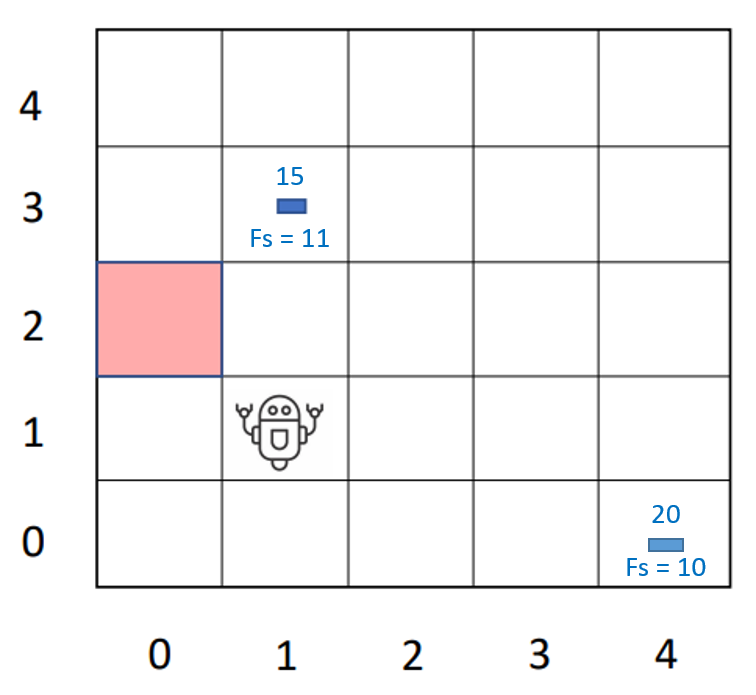
\includegraphics[width=0.9\linewidth]{Images/strategy.png}
    \caption{Pickup strategy}
    \captionsetup{font=footnotesize}
    \caption*{The number on top of the parcels is the current score, while the $Fs$ value is the final score. The red tile is the base. The agent will pickup the nearest parcel, even though the other one has a higher score currently}
    \label{fig:pickup}
\end{figure}

The desires list is then sorted by score, and the one with the highest score becomes the current intention.

% Parlare della possibile riconsiderazione delle parcel se vediamo altri agenti vicini
All the intentions are immediately transformed into an action, preceded by a planning phase, except for the \texttt{pickup} intention.
If the agent detects that another agent is going to get to the parcels faster them itself, it discard that intention and picks the second best one, perfoming again the checks if it is another \texttt{pickup} intention.
The pseudo-code for the \textit{agent-check} is the following:

\begin{lstlisting}[caption={Opponent agents checks}]
if a senses another agent:
    if agent is closer than a:
        if agent is 1 tile away from parcel OR going towards the parcel:
            discard parcel and pick next intention
\end{lstlisting}



If the opponent agent is next to the parcel it is assumed to pick up that parcel. The \textit{"going towards the parcel"} part is computed by analyzing the direction in which the agent is going, with respect to the parcel location.



\subsection{Actions}

The agent moves continuously in the map. Each path is calculated before acting, in a \textit{planning-like} phase, with the $A^*$ algorithm. 

\subsubsection*{Pickup}
% Spiegare cosa fa l'agent quando vuole fare pickup
The agent performs the \texttt{pickup} action by going to the location of the parcel and then picking it up.

\subsubsection*{Deposit}
% Spiegare cosa fa l'agent quando vuole fare deposit
The deposit intention is fulfilled by going to the nearest available home and deposit all of the carried parcels, and removing them from the memory.

\subsubsection*{Explore}
% Parlare di come avviene l'explore e il camping
If the selected intention is to \texttt{explore}, then the agent selected a reachable random spawn tile and goes to that location. If the map is \textit{sparse}, it stays on the same cell from a small period of time, waiting for a parcel to spawn.
The sparseness of the map is calculated at the beginning, based on a proportion between spawn tiles and total tiles in the map, and also spawn tiles and the maximum number of parcels present in the map at the same time.

\subsubsection*{Opponents handling}
% Spiegare come gestiamo gli avversari (che cambiamo strada se lo vediamo vicino)
All the movements are preceded by check, that verifies if the path to the agent's destination is clear, that is if no other agents are blocking that path.
If the agent sees another agent in the next cell along its path, it waits a configurable amount of time (which can also be zero seconds). If the path is still obstructed afterwards, it calculates a new path to its destination, excluding the tile where the opponent agent is standing.

\subsection{Results in the Challenge 1}

We placed 7\textsuperscript{th} out of 20 teams. During the live matches, we  noticed that every time we issued a movement command: our agent incurred a penalty due to sending a new command before the server had applied the previous one \footnote{During offline testing we did not encounter these synchronization issues.}. To solve this, we introduced a boolean flag \texttt{isMoving} in our \texttt{Agent} class, which is set to \texttt{true} immediately before sending any movement command and reset to \texttt{false} once the move completes:

\begin{lstlisting}[language=JavaScript,caption={Setting \texttt{isMoving} before and after moves}]
// Before moving:
this.isMoving = true;

await moveAndWait(this.client, this.me, dir);

// After move confirmation:
this.isMoving = false;
\end{lstlisting}

Thanks to this change, in \textit{Challenge 2} both agents no longer incurred movement penalties.
